% \begin{figure*}[t]
%     \centering
%     \begin{tikzpicture}
%         % Fourth column
%         \draw[thick] (13.5,0) rectangle (17.5,3);
%         \node at (15.5,1.5) {\normalsize{\textbf{(d)}} \small{Schema of our Model.}};
%     \end{tikzpicture}
%     \caption{Bouldering Illustrations.}
%     % \label{fig:four_columns}
% \end{figure*}

\begin{figure*}[t]
    \centering
    \begin{minipage}{0.49\textwidth}
        \centering
        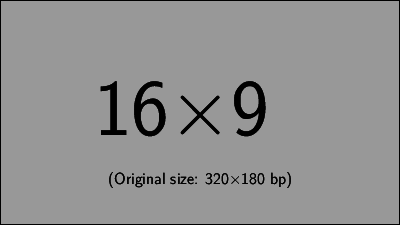
\includegraphics[width=\textwidth]{assets/mwe/example-image-16x9}
        \caption{Local Temporal Modeling}
        \label{figure:local-temporal-modeling}
    \end{minipage}
    \hfill
    \begin{minipage}{0.49\textwidth}
        \centering
        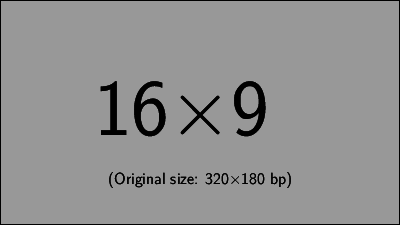
\includegraphics[width=\textwidth]{assets/mwe/example-image-16x9}
        \caption{Global Temporal Modeling}
        \label{figure:global-temporal-modeling}
    \end{minipage}
\end{figure*}

\section{Our Approach}

Explain the general idea with the feature extractor and other things.

Create an nice big to clearly explain the approach.

\todo[inline]{Reference the figure illustrating our model / base approach.}

Here we'll describe the approach we decided to take. First of all we'll state all the constraints we are faced with: Limited Computing Power (only my laptop), Limited Dataset size (only 8 unique videos), Limited time (4 Months for the research project).

And based on the constraints stated above we'll justify the choice of the approach which is to use a pre-existing model and fine tune it on our dataset.

Then we'll describe the different variants of our approach which are:
1- hand made feature extraction and selection.
2- automatic using a pre-trained model that is supposed to do that by extracting the hidden layers features.

And here we'll talk about the different types feature extractors:
- Frame by frame based.
- Sequence.
We need to develop, give examples, etc.

Than we'll talk about the possible ways of treating the features of the frame by frame feature extractor and the fact that there is nothing to do for the sequence feature extractor:
- We either take the average.
- Concatenate to make them look like a giant feature.
- Add them.
- Use a linear layer to combine them.
- Use an LSTM to temporally link them and create the temporal dependence and come up with a feature.
Cite which of the ways is recommended in which paper. Cite which one we used. Cite the drawbacks and advantages of each one.
Give examples for each model and feature cases, for example for yolo it come up to taking the average position.

Now talk about the different models that we can use to perform classification.
- LSTM on a sequence to sequence, like direct mapping not in encoder - decoder mode.
- LSTM in encoder-decoder mode.
- Simple linear layer.
- Transformer.

\subsection*{Considered Variants}

\subsection{Local Temporal Modeling}
Describe and illustrate. Explain the origin, the need, the pros and the cons.
\begin{figure*}[h]
    \centering
    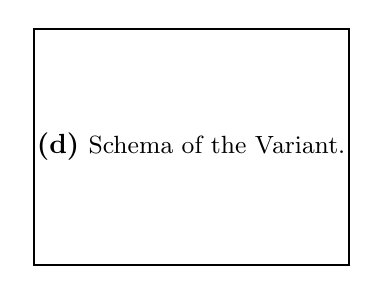
\begin{tikzpicture}
        % Fourth column
        \draw[thick] (13.5,0) rectangle (17.5,3);
        \node at (15.5,1.5) {\normalsize{\textbf{(d)}} \small{Schema of the Variant.}};
    \end{tikzpicture}
    \caption{Bouldering Illustrations.}
    % \label{fig:four_columns}
\end{figure*}

\subsection{Global Temporal Modeling}

\subsection{\textbf{Averaging + LSTM Sequence - Sequence}}
Describe and illustrate. Explain the origin, the need, the pros and the cons.
\begin{figure*}[h]
    \centering
    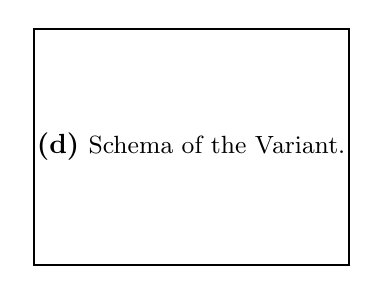
\begin{tikzpicture}
        % Fourth column
        \draw[thick] (13.5,0) rectangle (17.5,3);
        \node at (15.5,1.5) {\normalsize{\textbf{(d)}} \small{Schema of the Variant.}};
    \end{tikzpicture}
    \caption{Bouldering Illustrations.}
    % \label{fig:four_columns}
\end{figure*}

\subsection{\textbf{Averaging + LSTM Encoder - Decoder}}
Describe and illustrate. Explain the origin, the need, the pros and the cons.
\begin{figure*}[h]
    \centering
    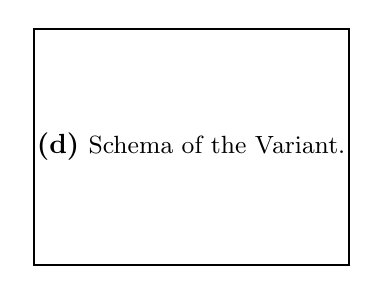
\begin{tikzpicture}
        % Fourth column
        \draw[thick] (13.5,0) rectangle (17.5,3);
        \node at (15.5,1.5) {\normalsize{\textbf{(d)}} \small{Schema of the Variant.}};
    \end{tikzpicture}
    \caption{Bouldering Illustrations.}
    % \label{fig:four_columns}
\end{figure*}

\subsection{\textbf{LSTM Modeling + LSTM Encoder - Decoder}}
Describe and illustrate. Explain the origin, the need, the pros and the cons.
\begin{figure*}[h]
    \centering
    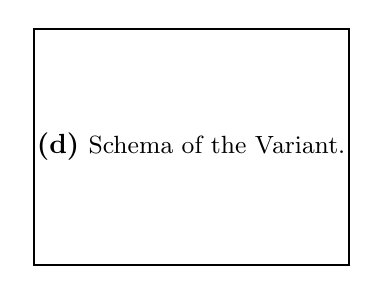
\begin{tikzpicture}
        % Fourth column
        \draw[thick] (13.5,0) rectangle (17.5,3);
        \node at (15.5,1.5) {\normalsize{\textbf{(d)}} \small{Schema of the Variant.}};
    \end{tikzpicture}
    \caption{Bouldering Illustrations.}
    % \label{fig:four_columns}
\end{figure*}